% ЕМТ 2025, XII клас — точен LaTeX препис от официалните файлове в Klasirane.com.
% Условия: https://klasirane.com/api/competitions/EMT/All/2025/12%20%D0%BA%D0%BB/probs
% SHA-256 (условия): 6ec1704151066ed81880089b9fad357245a9f89d5a225698bc9a9ddb34a0ed35
% Решения: https://klasirane.com/api/competitions/EMT/All/2025/12%20%D0%BA%D0%BB/sol
% SHA-256 (решения): 3b00417b65a93e3abbadd4aee0a0269d6d9acb2d9b2a73a6b3bb5411b7bf8b84
% Точковите оценки, правописът, формулировките и видимите печатни грешки са запазени от източника.
% Файлът с условията е едностранично сканирано изображение; видимата страница е проверена пряко.

Задача 12.1. Да се определят всички възможни стойности на израза $x^3+y^2+z$, където $x$, $y$ и $z$ са реални неотрицателни числа, за които $x^2+y^2+z^2=1$.

Решение. Имаме, че
$$x^3+y^2+z\le x^2+y^2+z=1-z^2+z=-\left(\frac12-z\right)^2+\frac54\le\frac54,$$
както и
$$x^3+y^2+z\ge x^3+y^2+z^2=x^3-x^2+1.$$
От друга страна функцията $f(x):=x^3-x^2+1$ изпълнява $f'(x)=3x^2-2x$, откъдето следва, че $f$ има точно един локален минимум в $[0,1]$, а именно $x=\frac23$, т.к $f'(x)>0$ за $x<0$, $f'(x)<0$ за $x\in(0,\frac23)$ и $f'(x)>0$ за $x\in(\frac23,1]$. Така получаваме, че $x^3+y^2+z\ge f(x)\ge f(\frac23)=\frac{23}{27}$. От съображения за непрекъснатост функцията $f(x)$ приема всички стойности в интервала $[\frac{23}{27},1]$, а функцията $g(z):=1-z^2+z$ приема всички стойности в $[1,\frac54]$, което означава, че всяка стойност $a\in[\frac{23}{27},\frac54]$ се достига – ако $a\le1$ избираме $x_0$, т.че $f(x_0)=a$ и полагаме $(x,y,z)=(x_0,\sqrt{1-x_0^2},0)$, а ако $a>1$ избираме $z_0\in[0,1]$, за което $g(z_0)=a$ и полагаме $(x,y,z)=(0,\sqrt{1-z_0^2},z_0)$. Еквивалентно последната стъпка може да се замени с обобщение на теоремата за междинните стойности, като е необходимо да се отбележи, че множеството $\{(x,y,z)\in\mathbb R^3:x,y,z\in[0,1],x^2+y^2+z^2=1\}$ е свързано и бъдат посочени стойности на $x,y,z$, за които долната и горната граница на израза се достигат.

Оценяване. (6 точки) 3 т. за $f(x)\ge\frac{23}{27}$; 1 т. за $x^3+y^2+z\le\frac54$; 2 т. за довършване.

Задача 12.2. Даден е остроъгълен и разностранен $\triangle ABC$ с описана окръжност $\omega$ и център на вписаната окръжност $I$. Нека $CI\cap\omega=\{C,M\}$ и нека $X$ е такава точка от лъча $MI$, че $MX=\frac{CI}{2}$. Ако точката $N$ е среда на отсечката $BC$, то да се докаже, че $\angle IAX=\angle INX$.

Решение. Нека точка $J$ е центърът на външновписаната окръжност на $\triangle ABC$ срещу върха $C$. Имаме, че $X$ е среда на $CJ$, т.к $IM=MJ$. От друга страна $\triangle AJC\sim\triangle IBC$, т.к.
$$\angle AJC=\angle IBC=\frac{\angle ABC}{2}$$
и
$$\angle ACJ=\angle ICB=\frac{\angle ACB}{2}.$$
Да отбележим, че точките $X$ и $N$ са съответни елементи в двата триъгълника, откъдето следва, че $\angle NIC=\angle XAC$.

Оттук нататък задачата може да се реши по няколко начина:

Първи начин. $XN\parallel BJ$ като средна отсечка в $\triangle CBJ$, откъдето $\angle NXI=\angle JBI=\angle CAI$. Така
$$\angle INX=\angle CIN-\angle IXN=\angle CAX-\angle IAC=\angle XAI.$$

Втори начин. Ако $NI\cap AX=P$, то
$$\angle PAC+\angle PIC=\angle XAC+180^\circ-\angle NIC=180^\circ,$$
т.е. точките $A,P,I,C$ лежат на една окръжност. Оттук следва, че $\angle XPN=\angle ACI=\angle XCN$, т.е $P,X,C,N$ са на една окръжност. Следователно $\angle XNI=\angle PCI=\angle IAX$, като последното следва от фактът, че $APIC$ е вписан.

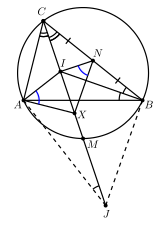
\includegraphics[max width=0.48\textwidth, alt={Официалната фигура към решение 12.2 с триъгълника ABC и точките I, J, M, N и X}, center]{assets/12-2-geometry.svg}

Оценяване. (6 точки) 2 т. за $X$ е среда на $CJ$; 1 т. за $\triangle AJC\sim\triangle IBC$; 1 т. за отбелязване, че $X$ и $N$ са съответни елементи; 2 т. за довършване

Задача 12.3. Нека $A_1,\ldots,A_{2025}$ са (не непременно различни) точки в $\mathbb R^3$. Да се определи максималният брой тройки индекси $1\le i<j<k\le2025$, за които точките $A_i,A_j,A_k$ образуват равностранен триъгълник със страна 1.

Отговор. $506^2\cdot2027=518\,984\,972$.

Решение. Ще наричаме тройка индекси $1\le i<j<k\le2025$ \emph{хубава}, ако $\triangle A_iA_jA_k$ е равностранен със страна 1.

Пример за конфигурация с $506^2\cdot2027$ хубави тройки индекси е правилен тетраедър $ABCD$, за който всички точки $A_i$ са разпределени равномерно във върховете му, т.е $A_i\equiv A$ за $i=1,2,\ldots,506$; $A_i\equiv B$ за $i=507,\ldots,1012$; $A_i\equiv C$ за $i=1013,\ldots,1518$ и $A_i\equiv D$ за $i=1519,\ldots,2025$. Това дава общо
$$506^3+3\cdot506^2\cdot507=506^2\cdot2027$$
хубави тройки индекси.

Да разгледаме конфигурация от точки $A_1,A_2,\ldots,A_{2025}$, която максимизира броя тройки с исканото свойство и да допуснем, че има две точки $A_i,A_j$, които са на разстояние различно от 1. БОО можем да приемем, че $A_i$ участва в повече равностранни триъгълници със страна 1 от $A_j$. Тогава, ако преместим $A_j$ в $A_i$, то общият брой равностранни триъгълници със страна 1 не намалява, т.к $A_i$ и $A_j$ не участват заедно в равностранен триъгълник със страна 1. Следователно съществува максимална конфигурация, за която разстоянието между всеки две точки $A_i$ и $A_j$ е или 0 или 1.

Да отбележим, че т.к не съществува множество от 5 точки в $\mathbb R^3$, за което разстоянието между всеки две от тях е равно на 1, то съществува максимална конфигурация, за която всички точки се намират във върховете на правилен тетраедър $ABCD$.

Нека $a,b,c,d\in\mathbb Z_{\ge0}$ са бройката точки, намиращи се в $A,B,C,D$ съответно. Тогава общият брой хубави тройки индекси е
$$abc+bcd+cda+dab=ab(c+d)+cd(a+b)=bc(a+d)+ad(b+c)=ac(b+d)+bd(a+c),$$
като да отбележим, че е в сила $a+b+c+d=2025$.

БОО нека $a\ge b\ge c\ge d$. Ако $a-d\ge2$, то ако заменим $a$ с $a-1$ и $d$ с $d+1$, получавайки
$$\begin{aligned}
bc(a+d)+(a-1)(d+1)(b+c)&=bc(a+d)+(ad+a-d-1)(b+c)\\
&\ge bc(a+d)+(ad+1)(b+c)\\
&>bc(a+d)+ad(b+c),
\end{aligned}$$
т.е в максимална конфигурация имаме $|a-d|\le1$, откъдето следва, че $\{a,b,c,d\}=\{506,507\}$.

Оценяване. 0 точки за отговор; 1 т. за разглеждане на конфигурация, в която всички точки са във върховете на правилен тетраедър; 1 т. за вярно балансиране на върховете в тетаредъра и вярно пресмятане на отговора;

Оценка от горе: 1 т. за ясно твърдение, че в пространството няма 5 точки, всеки две от които са на разстояние 1; 1 т. за идеята за залепянето на точки на разстояние различно от 1; 3т. за довършване.

Други частични резултати (неадитивни с тези за горната оценка): До 2 точки за оценка от вида $cn^3$ за някое $c>\frac1{16}$ в зависимост от стойността на $c$. Например $c=\frac16$ носи 0 точки $c=\frac7{60}$ носи 2 точки.

Задача 12.4. Съществува ли естествено число $n$ с точно 4500 делители, за което десетичният запис на $\sqrt n$ започва с 2025 деветки след десетичната запетая, т.е $\sqrt n=A,\underbrace{99\ldots9}_{2025}\ldots$, за някое естествено число $A$?

Отговор. Да!

Решение. Първо ще докажем следната

Лема. Ако $M\in\mathbb N$, то съществуват безбройно много естествени числа $k$, за които интервалът $(k^2,(k+1)^2)$ съдържа поне $M$ прости числа.

Доказателство. Да отбележим, че е достатъчно да докажем, че поне едно $k$ съществува за всяко $M$, т.к $k$-то, което работи за $m\ge M$, работи и за $M$, откъдето можем да конструираме безкрайна редица от $k$-та за дадено $M$. Да допуснем, че за всяко $k$ интервалът съдържа $(k^2,(k+1)^2)$ най-много $M$ прости числа. Добре известно е, че $\sum_{p-\text{просто}}\frac1p=\infty$, откъдето следва, че
$$\infty=\sum_{p-\text{просто}}\frac1p=\sum_{k=1}^{\infty}\sum_{p\in(k^2,(k+1)^2)}\frac1p\le\sum_{k=1}^{\infty}\frac{M}{k^2}\le2M,$$
което е противоречие. С това лемата е доказана.

Ще докажем следното по-общо твърдение:

Ако $\varepsilon>0$ и $a$ е нечетно, то съществува естествено число $n$ с $4a$ делители, за което дробната част на $\sqrt n$ изпълнява $\{\sqrt n\}>1-\varepsilon$.

Доказателство. От лемата следва, че можем да намерим интервал $(k^2,(k+1)^2)$, съдържащ поне $2l+1$ прости числа, където $l:=\left\lceil\frac{2^a}{\varepsilon}\right\rceil$. Нека тези прости числа са
$$k^2<q_0<q_1<q_2<\cdots<q_{2l}<(k+1)^2.$$
Следователно имаме
$$2k\ge q_{2l}-q_0=\sum_{i=1}^l(q_{2i}-q_{2(i-1)})\ge l\min_{i\le l}(q_{2i}-q_{2(i-1)}),$$
т.е съществува $i$, за което $q_{2i}-q_{2(i-1)}\le\frac{2k}{l}$. За $p:=q_{2i}$ и $q:=q_{2i-1}$ имаме, че
$$\frac{p+q}{2}-\sqrt{pq}=\frac{(\sqrt p-\sqrt q)^2}{2}=\frac12\cdot\left(\frac{p-q}{\sqrt p+\sqrt q}\right)^2\le\frac12\cdot\left(\frac{2k}{l}\cdot\frac1{2k}\right)^2\le\frac1{l^2}.$$

Сега нека изберем $n:=2^{a-1}pq$. Имаме, че
$$\sqrt n-2^{\frac{a-3}{2}}(p+q)=2^{\frac{a-1}{2}}\left(\sqrt{pq}-\frac{p+q}{2}\right)\le\frac{2^{\frac{a-1}{2}}}{l^2}<\varepsilon.$$
Оттук твърдението следва, както и задачата след избор на $a=1125$, $\varepsilon=10^{-2026}$.

Оценяване. (7 точки) 1 т. за търсене на решение от вида $Apq$, където $A$ е фиксирано с $45\cdot25$ делители; 2 т. за намиране на близки прости числа $p$ и $q$ чрез лемата или друг вариант на PNT; 4 т. за довършване.
